\RequirePackage[l2tabu, orthodox]{nag}

\documentclass[10pt]{scrartcl}
% \documentclass[10pt]{article}
\usepackage[T1]{fontenc}
\usepackage{amsmath,amsfonts,amssymb}
\usepackage{mathtools}
\usepackage{color,soul}
\usepackage[margin=2cm]{geometry}
\usepackage{enumerate}
\usepackage{graphicx}
\usepackage[colorlinks=true,urlcolor=blue]{hyperref}
\usepackage{floatrow}
\usepackage{deluxetable}
\usepackage{verbatim}
\usepackage{fancyvrb}
\usepackage{listings}
\usepackage{calc}
\usepackage[font=small]{caption}
\usepackage[font=scriptsize]{subcaption}
\usepackage[activate={true,nocompatibility},final,tracking=true,kerning=true,spacing=true,factor=1100,stretch=10,shrink=10]{microtype}
\SetTracking{encoding={*}, shape=sc}{40}

\floatsetup{ 
  heightadjust=object,
  valign=t
}

\definecolor{Light}{gray}{.90}
\sethlcolor{Light}

\title{Multi-Sun Centroiding}
\author{Jeren Suzuki}
\date{Last Edited \today}

\begin{document}

\maketitle
\pagenumbering{Roman}
\tableofcontents
\clearpage
\pagenumbering{arabic}

\section{Introduction} % (fold)
\label{sec:introduction}
\hl{\texttt{beta.pro}} loads an image with any combination from a list of suns below and returns the center positions of the whole suns only. The only user-interaction is the selection of which region to analyze. The rest of the process is automatic. 

\begin{itemize}
    \item R1 \& R2
    \item R2 \& R3
    \item R1 \& R3
    \item R1 \& R2 \& R3
    \item R1 \& partial R2
    \item R1 \& partial R3
    \item R2 \& partial R3
    \item partial R1 \& R2
    \item partial R1 \& R3
    \item R1 \& partial R2 \& R3
    \item partial R1 \& R2 \& R3
    \item R1 \& partial R2 \& partial R3
    \item partial R1 \& partial R2 \& R3
    \item partial R1 \& R2 \& partial R3
\end{itemize}

Table \ref{structtable} breaks down the resulting strucutre of the centroiding program:\\

\begin{deluxetable}{cllllllll}
    \tablecaption{Final data structure of solar region}
    \tablecolumns{4}
    \tabletypesize{\scriptsize}
    \tablewidth{0pt}
    \tablehead{ 
      \colhead{Name} %
    & \colhead{Type} %
    & \colhead{Value} %
    & \colhead{Notes}
    }
    \startdata
    \hline
    XPOS
    & FLOAT
    & 210.522
    & Rough calculation using a simple masking method\\
    %
    YPOS
    & FLOAT
    & 166.702
    & ''\\
    %
    REG
    & INT
    & 1
    & Region ID \#: 1 is 100\%, 2 is 50\%, 3 is 25\%\\
    %
    THRESH
    & FLOAT
    & 106.000
    & Threshold calculated from sorting array and taking derivatives.\\ & & & Used in both finding rough X-Y center as well as the\\ & & & threshold for limb-fitting.\\
    %
    PARTIAL
    & FLOAT
    & 0.
    & Flag that determines if the solar region is cut off on the edge or not.\\ & & & 0 means that it is not cut off \\
    %
    XSTRIPS
    & STRUCTURE
    & -> WHOLEXSTRIPS Array[5]
    & Strucutre containing the strips of whole solar data\\ & & & bound by a cropped region chosen by XPOS and YPOS\\
    %
    YSTRIPS
    & STRUCTURE
    & -> WHOLEYSTRIPS Array[5]
    & ''\\
    %
    LIMBXSTRIPS
    & STRUCTURE
    & -> LIMBXSTRIPS Array[5]
    & LIMBSTRIPS contains a pair of arrays, ENDPOINTS and \\ & & & STARTPOINTS that mark the limbs of each strip of data from \\ & & & X/YSTRIPS\\
    %
    LIMBYSTRIPS
    & STRUCTURE
    & -> LIMBYSTRIPS Array[5]
    & ''\\
    %
    LIMBXPOS
    & FLOAT
    & 210.710
    & Center calculated from LIMBXSTRIPS\\
    %
    LIMBYPOS
    & FLOAT
    & 167.172
    & ''\\
    \enddata
\label{structtable}
\end{deluxetable}


% section introduction (end)

\section{Centroiding a Solar Image} % (fold)
\label{sec:centroiding_a_solar_image}

The current method to find the centers of any solar image is the following:

\begin{enumerate}
    \item Load Image
    \item Read parameters from pblock.txt
    \item Sort image and cut off top .1\% of pixels (top 1\% was actually too much)
    \item Smooth, take deriv, smooth again, take deriv again of sorted array, find peaks that correspond to difference solar regions and their thresholds
    \item Mask image above thresholds to find centers of every shape, regardless of partial or not
    \item Scan border of image looking for consecutive pixels above lowest threshold
    \item If more than 5 pixels in a row, marks x and y position and tags nearest solar center as ``partial''
    \item Crop remaining whole suns
    \item Extract 5 strips centered around cropped solar center for both X and Y direction
    \item Extract a pair of limb strips for each long strip
    \item Fit 2D polynomial to limb profile
    \item Mark position where fitted polynomial crosses threshold 
    \item Use positions to find chord lengths of sun
    \item Average midpoints of chords to find limb-fitted centers
    \item Using the limb-fitted centers, recrop the image so that every pixel in the image is part of the solar disk
    \item Analyze the cropped image for fiducials
    \item Using the fiducial positions, we compare the solar positions we calculated to a position defined by the physical setup.
    \item Not directly in the workflow, but we also use the solar centers to find the rotation angle/orientation of the setup. This kind of calculation is increasingly worse with less whole solar regions
    \item HMMMMMMMMMMMMMMMMMMMMMMMMMMMMMMMMMMMMMMMMMMMMM
\end{enumerate}

% section partial_suns (end)

\section{Issues} % (fold)
\label{sec:issues}
The current method of finding thresholds in the image is robust, yet slow. The problem doesn't lie in the second derivative, but the smoothing of the data so the derivaties return unusable data. As of now, the best smoothing filter is also the slowest, \hl{\texttt{ts\_smooth()}}. Figure \ref{smoothtest} shows the difference that \hl{\texttt{ts\_smooth()}} makes. smoothedarr is the sorted array soothed with \hl{\texttt{ts\_smooth()}}. The arrays look a \emph{LOT} worse if we use \hl{\texttt{smooth(sortedarray)}} instead of \hl{\texttt{ts\_smooth(sortedarray)}} (See Figure \ref{badsmooth}). \\

\begin{figure}[!ht]
    \ffigbox[][\FBheight]{%
    \begin{subfloatrow}[2]%
        \ffigbox[\FBwidth]%
       {%
       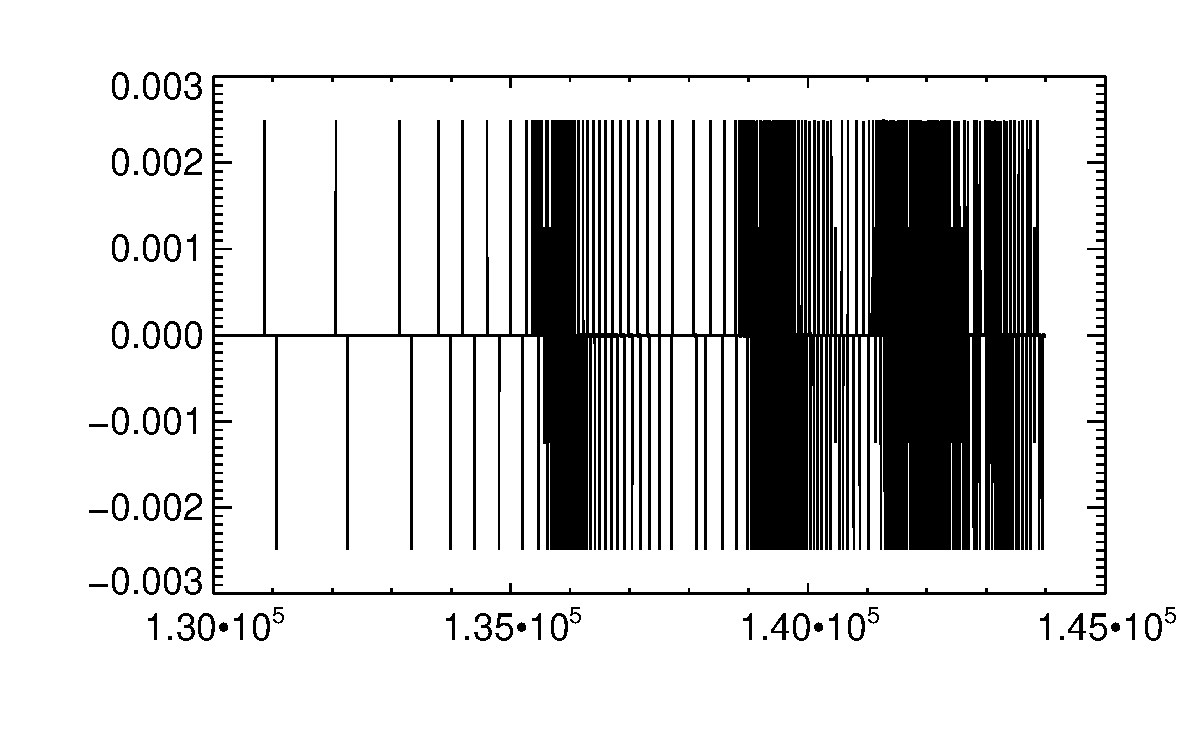
\includegraphics[width=.5\textwidth]{../plots_tables_images/firstsmoothonly.eps}%
       }%
       {%
       \caption{\hl{\texttt{deriv(deriv(smoothedarr))}}}%
       }%
        \ffigbox[\Xhsize]%
       {%
       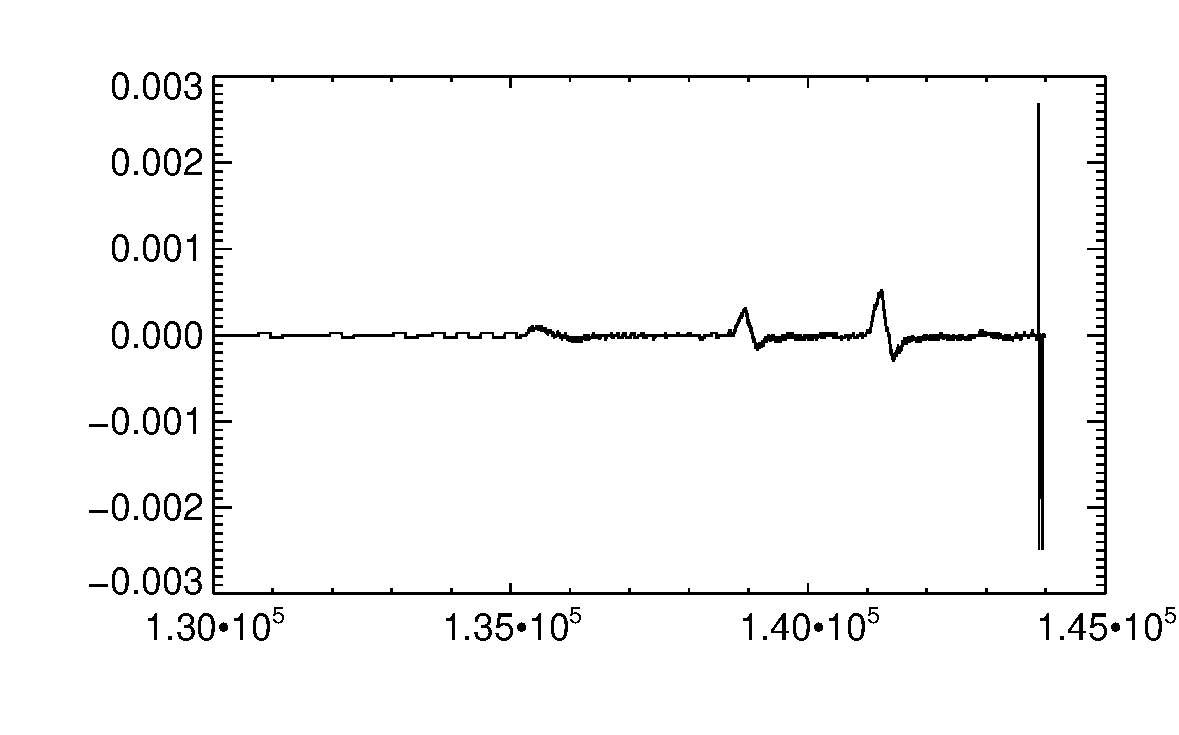
\includegraphics[width=.5\textwidth]{../plots_tables_images/nowrap.eps}%
       }%
       {%
       \caption{\hl{\texttt{deriv(smooth(deriv(smoothedarr)))}}}%
       }%
    \end{subfloatrow}}

    \ffigbox[][\FBheight]{%
    \begin{subfloatrow}[2]%
        \ffigbox[\FBwidth]%
       {%
       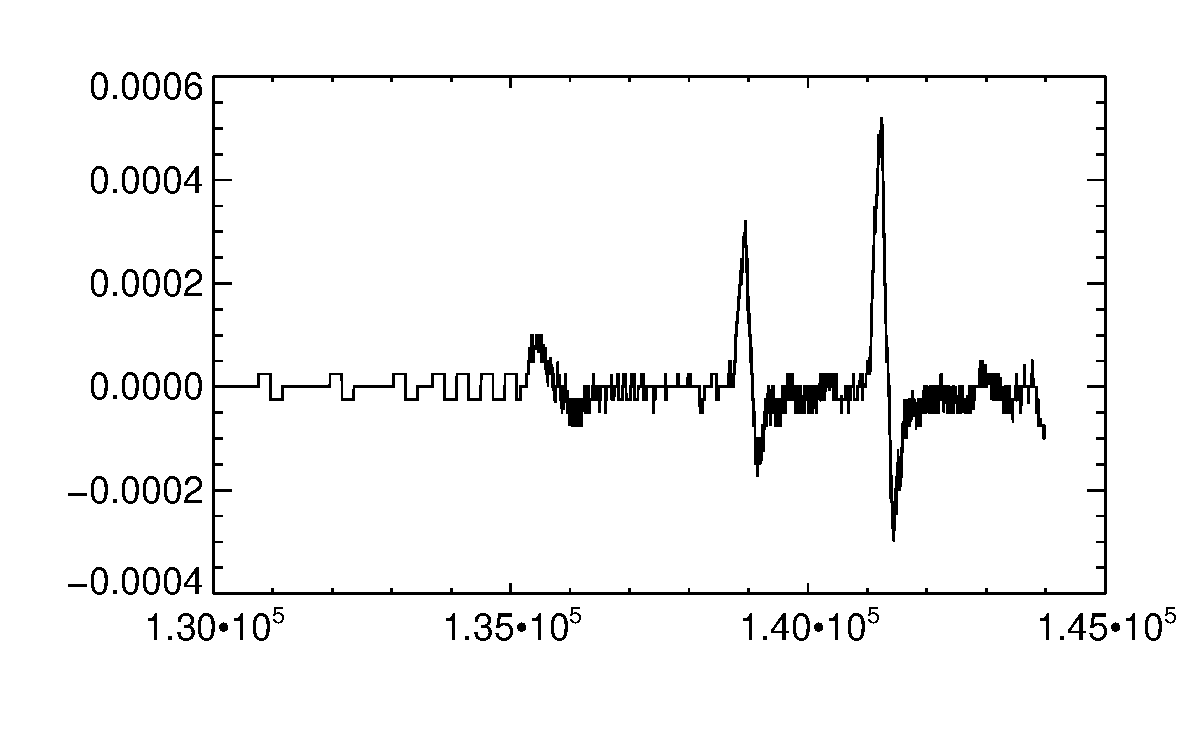
\includegraphics[width=.5\textwidth]{../plots_tables_images/justsmooth.eps}%
       }%
       {%
       \caption{\hl{\texttt{deriv(smooth(deriv(smoothedarr),/edge\_wrap))}}}%
       }%
        \ffigbox[\Xhsize]%
       {%
       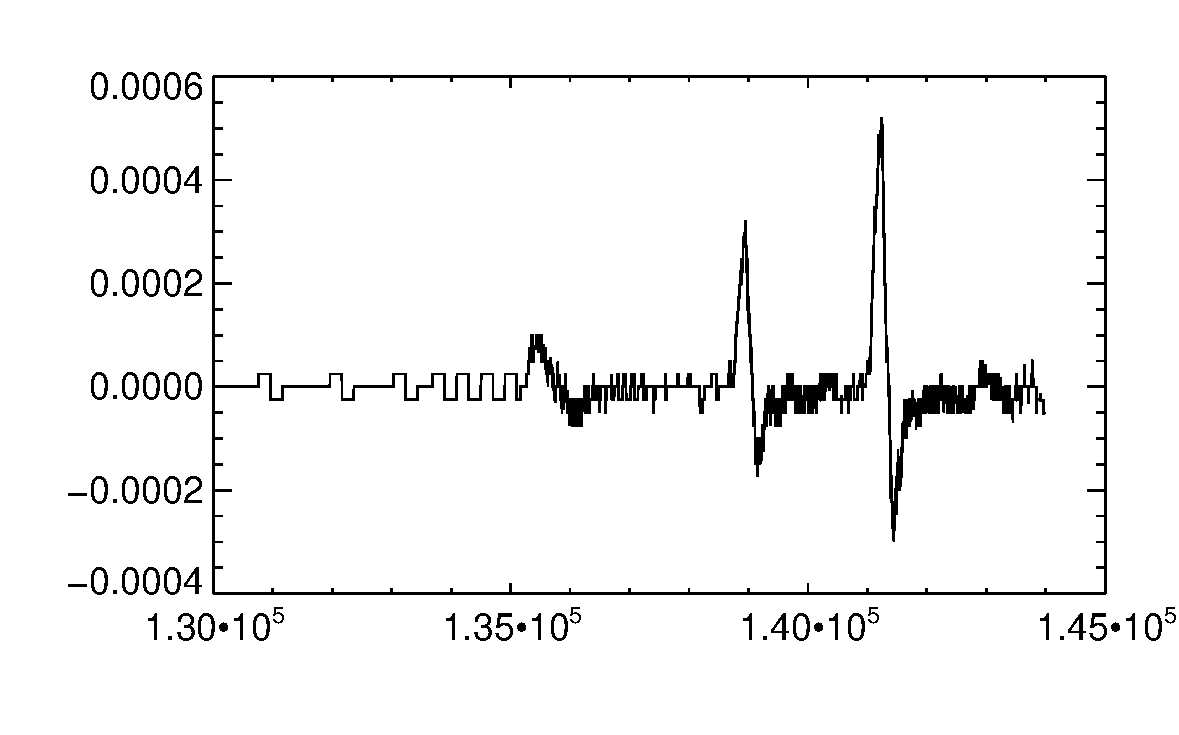
\includegraphics[width=.5\textwidth]{../plots_tables_images/doubletssmooth.eps}%
       }%
       {%
       \caption{\hl{\texttt{deriv(ts\_smooth(deriv(smoothedarr)))}}}%
       }%
    \end{subfloatrow}}

    \ffigbox[][\FBheight]{%
    \begin{subfloatrow}[2]%
        \ffigbox[\FBwidth]%
       {%
       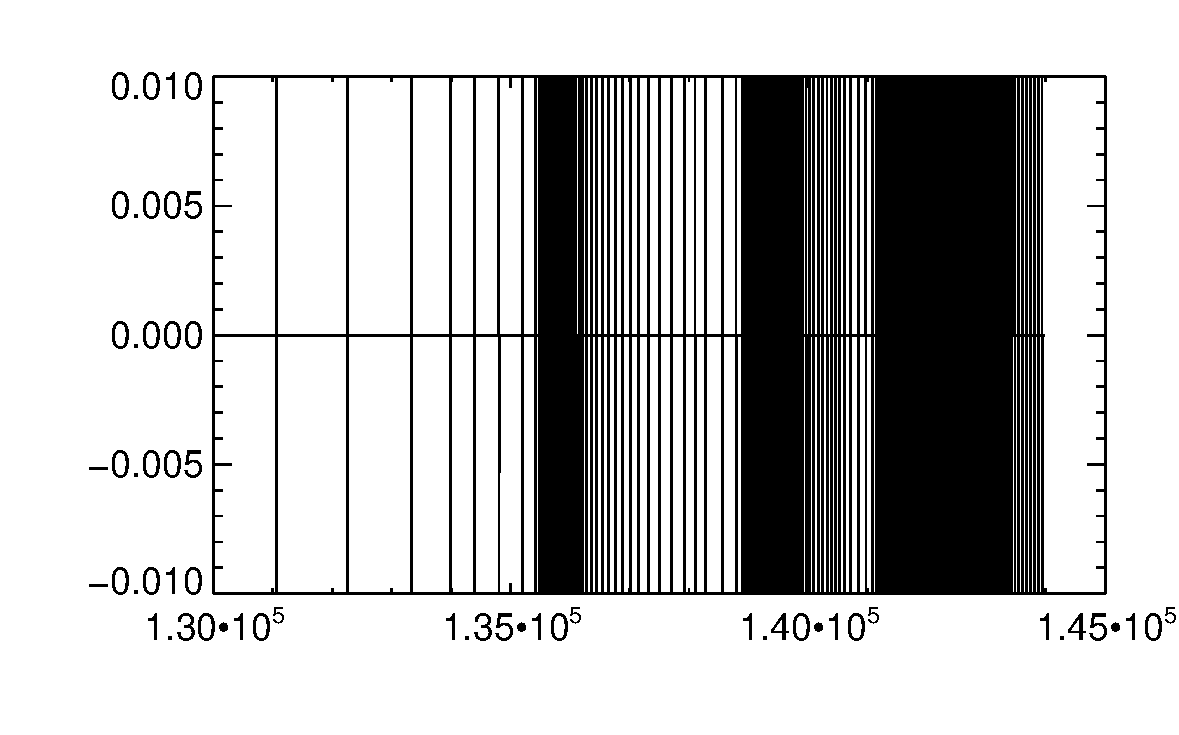
\includegraphics[width=.5\textwidth]{../plots_tables_images/sm_firstsmoothonly.eps}%
       }%
       {%
       \caption{\hl{\texttt{deriv(deriv(smooth(sortedarray)))}}}%
       }%
        \ffigbox[\Xhsize]%
       {%
       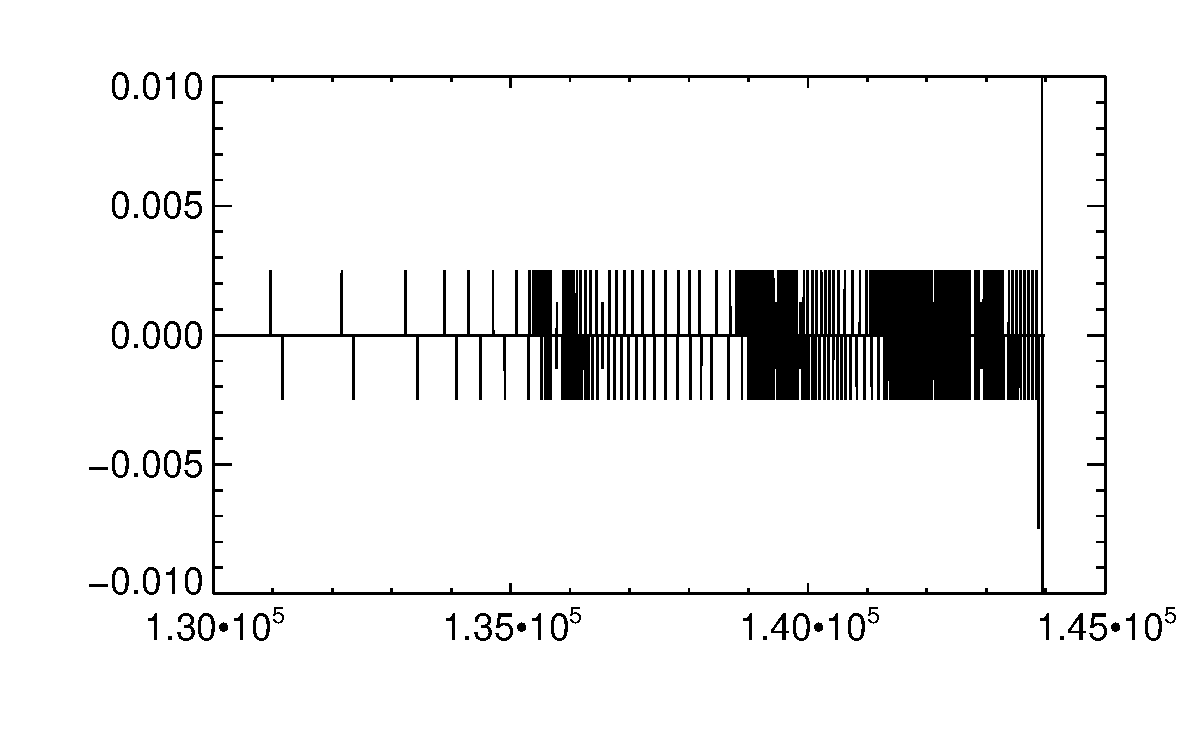
\includegraphics[width=.5\textwidth]{../plots_tables_images/sm_nowrap.eps}%
       }%
       {%
       \caption{\hl{\texttt{deriv(smooth(deriv(smooth(sortedarray))))}}}%
       }%
    \end{subfloatrow}}

        \ffigbox[][\FBheight]{%
    \begin{subfloatrow}[2]%
        \ffigbox[\FBwidth]%
       {%
       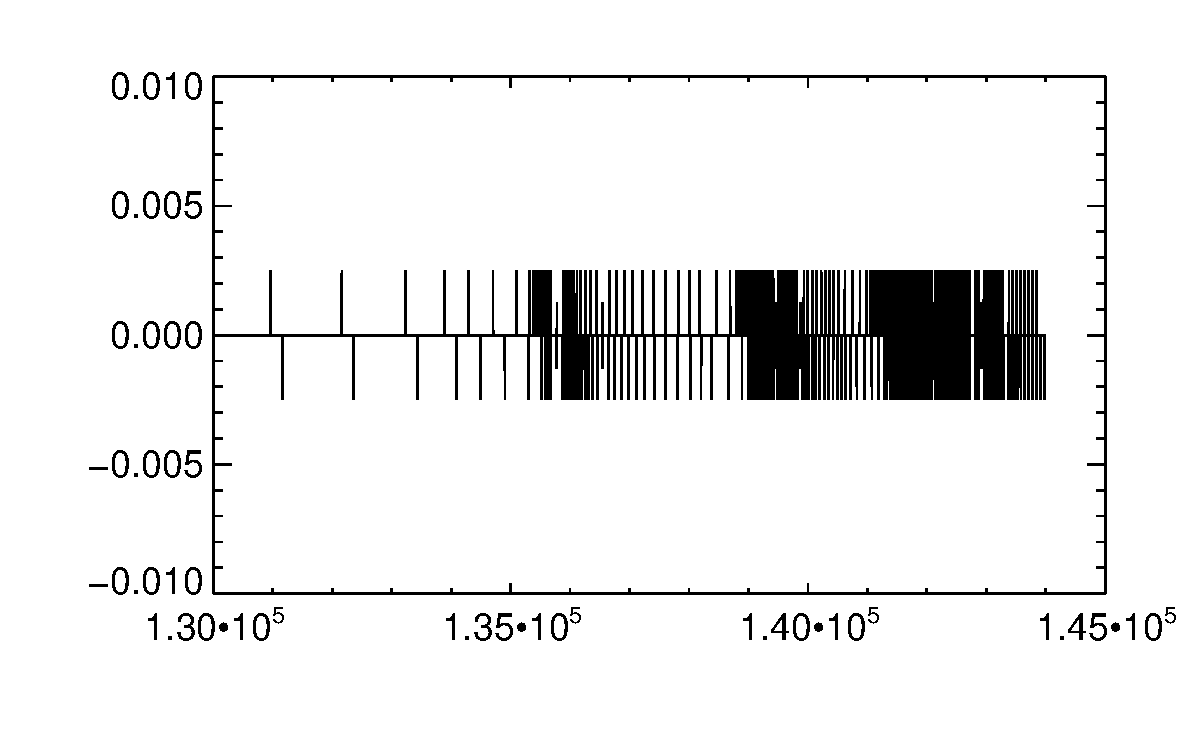
\includegraphics[width=.5\textwidth]{../plots_tables_images/sm_justsmooth.eps}%
       }%
       {%
       \caption{\hl{\texttt{deriv(smooth(deriv(smooth(sortedarray)),/edge\_wrap))}}}%
       }%
        \ffigbox[\Xhsize]%
       {%
       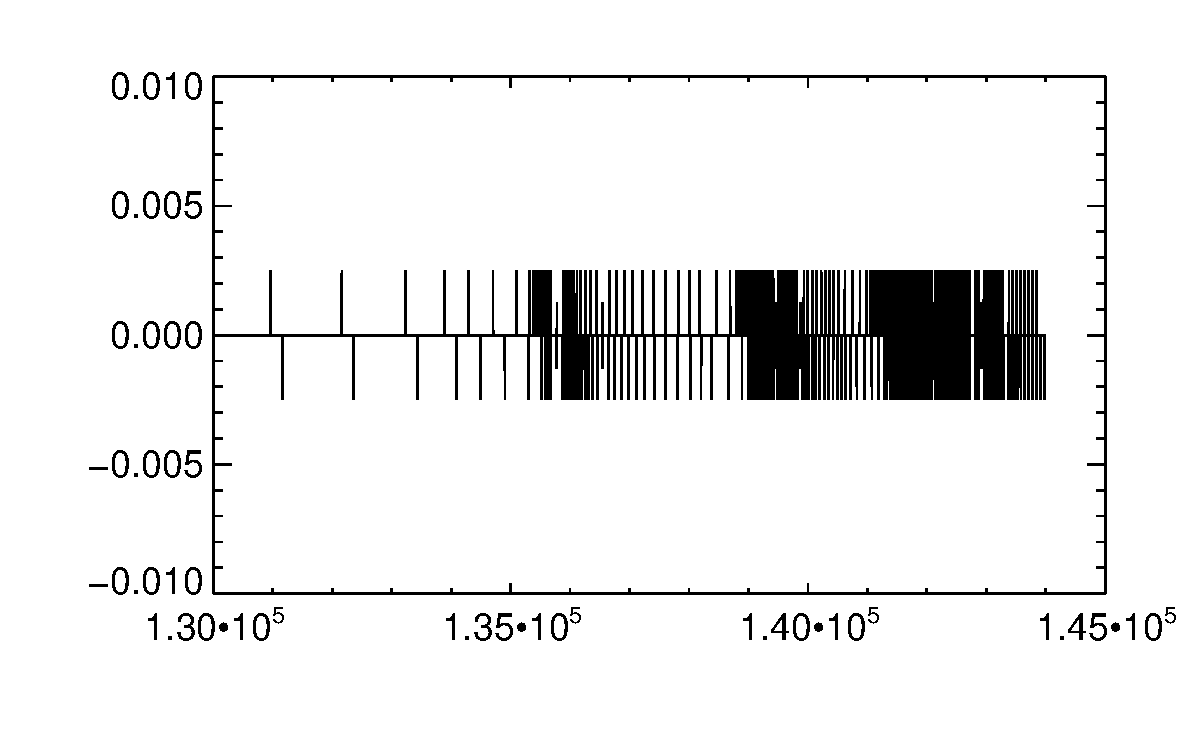
\includegraphics[width=.5\textwidth]{../plots_tables_images/sm_doubletssmooth.eps}%
       }%
       {%
       \caption{\hl{\texttt{deriv(ts\_smooth(deriv(smooth(sortedarray))))}}}%
       }%
    \end{subfloatrow}}
    {\caption{}\label{badsmooth}}%
\end{figure}

% \begin{figure}[!h]
%     \begin{center}
%     \begin{subfigure}[b]{.49\textwidth}
%         \centering
%         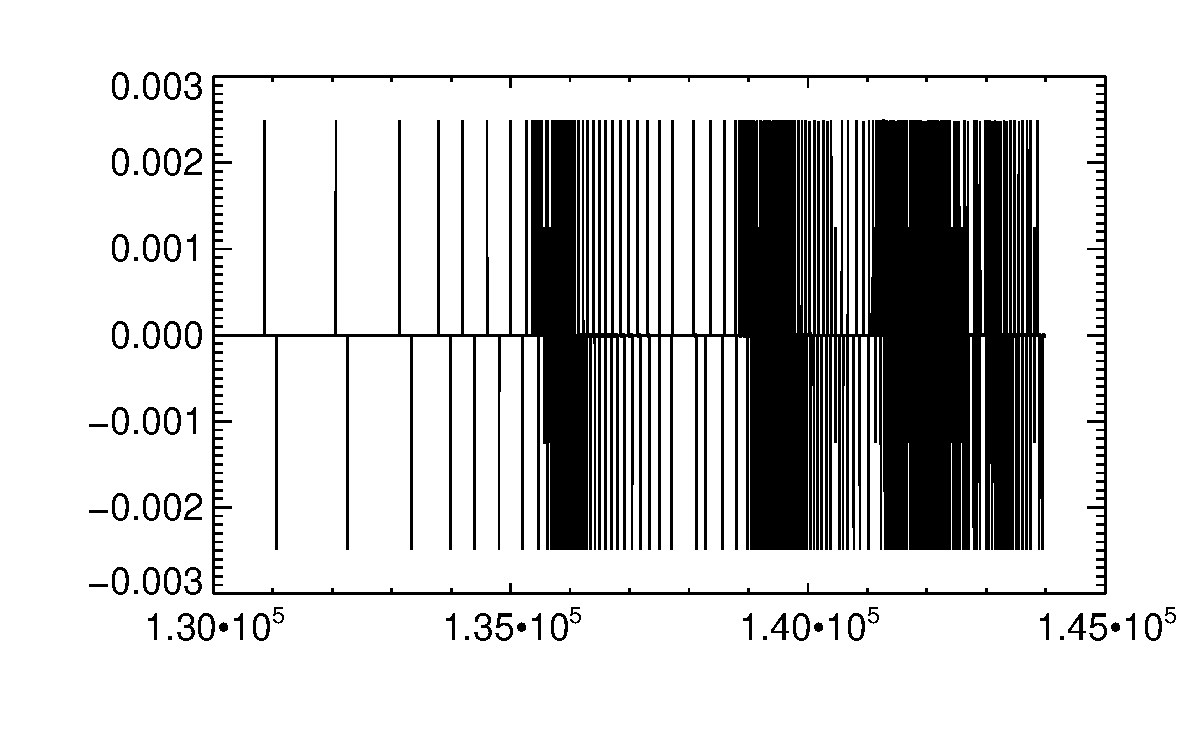
\includegraphics[width=1.\textwidth]{../plots_tables_images/firstsmoothonly.eps}
%         \caption{\hl{\texttt{deriv(deriv(smoothedarr))}}}
%     \end{subfigure}
%     \begin{subfigure}[b]{.49\textwidth}
%         \centering
%         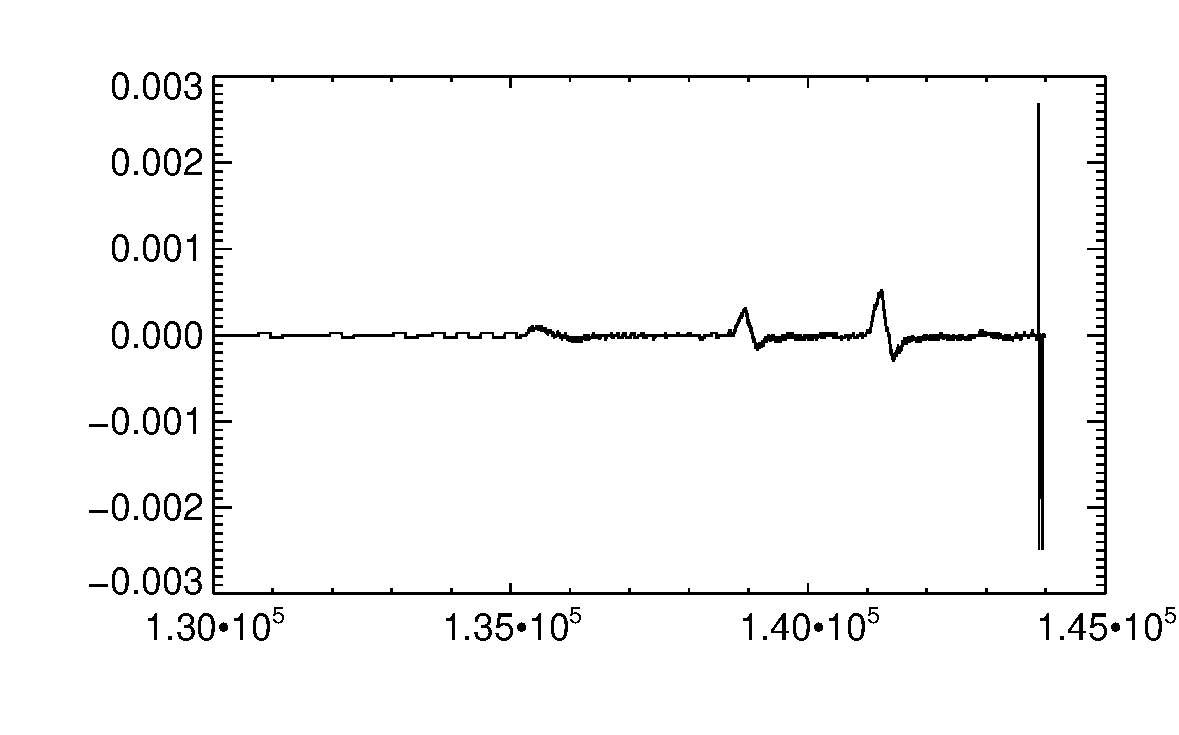
\includegraphics[width=1.\textwidth]{../plots_tables_images/nowrap.eps}
%         \caption{\hl{\texttt{deriv(smooth(deriv(smoothedarr)))}}}
%     \end{subfigure}

%    \begin{subfigure}[b]{.49\textwidth}
%         \centering
%         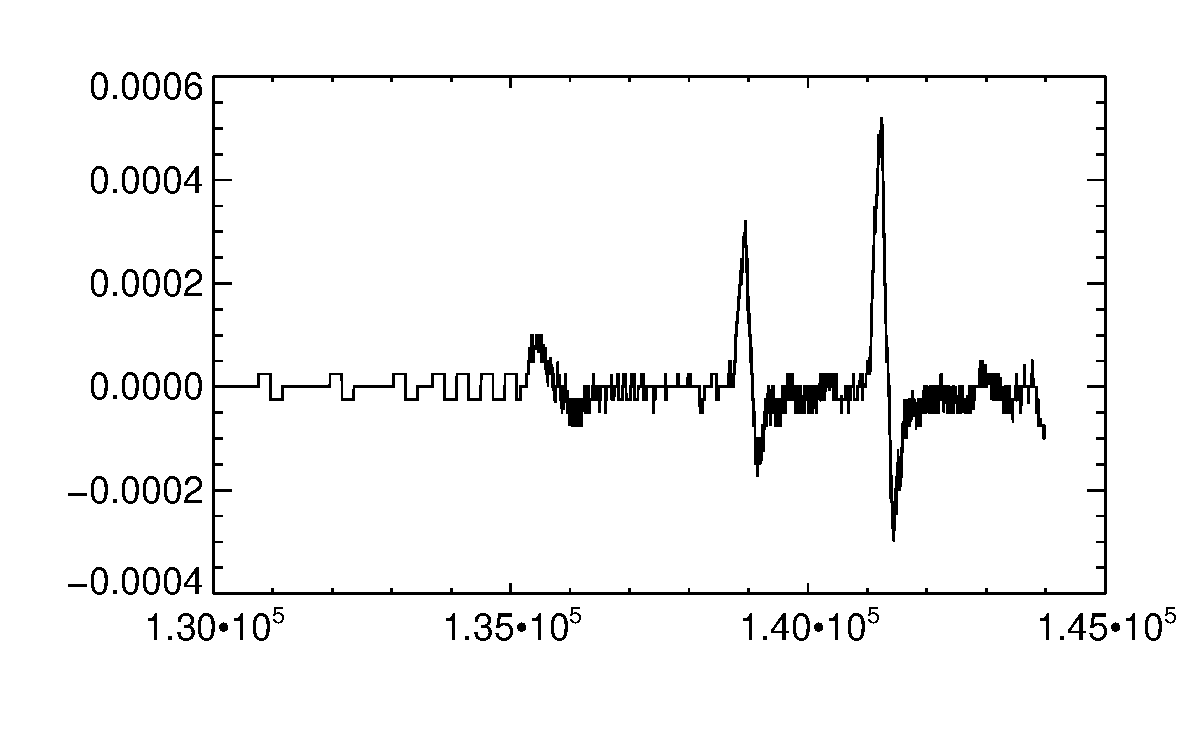
\includegraphics[width=1.\textwidth]{../plots_tables_images/justsmooth.eps}
%         \caption{\hl{\texttt{deriv(smooth(deriv(smoothedarr),/edge\_wrap))}}}
%     \end{subfigure}
%     \begin{subfigure}[b]{.49\textwidth}
%         \centering
%         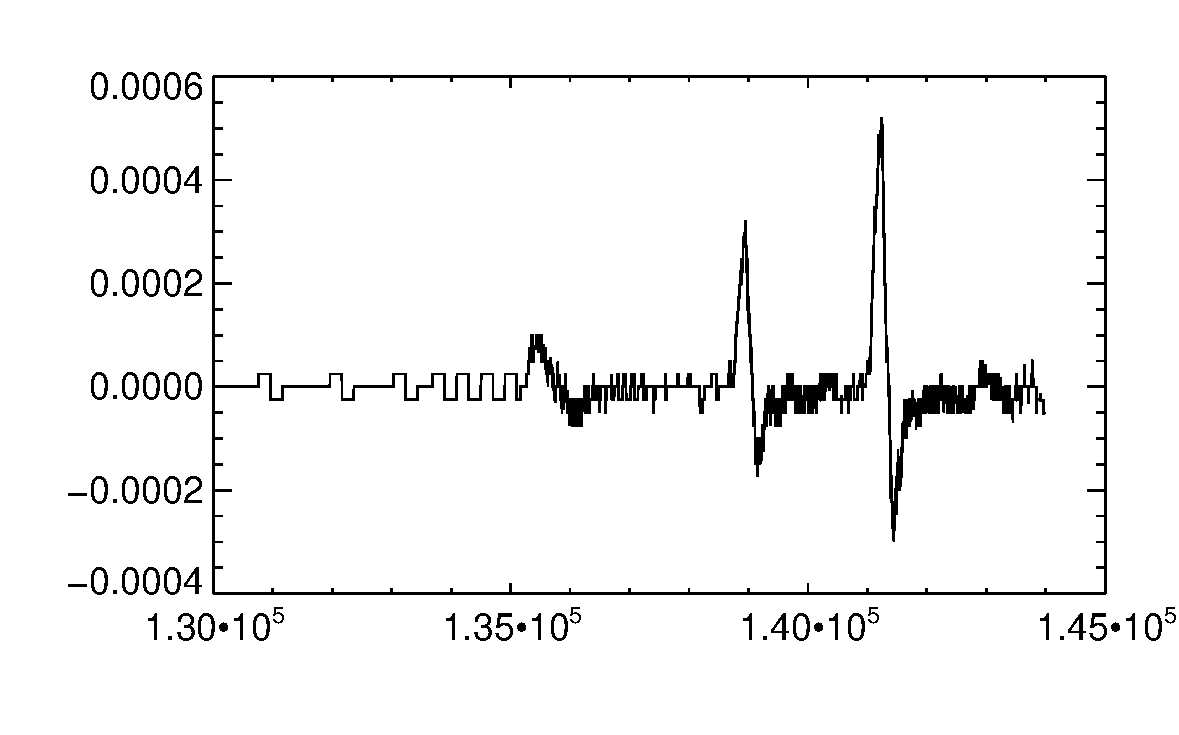
\includegraphics[width=1.\textwidth]{../plots_tables_images/doubletssmooth.eps}
%         \caption{\hl{\texttt{deriv(ts\_smooth(deriv(smoothedarr)))}}}
%     \end{subfigure}
%     \caption{}
%     \label{smoothtest}

%     \begin{subfigure}[b]{.49\textwidth}
%         \centering
%         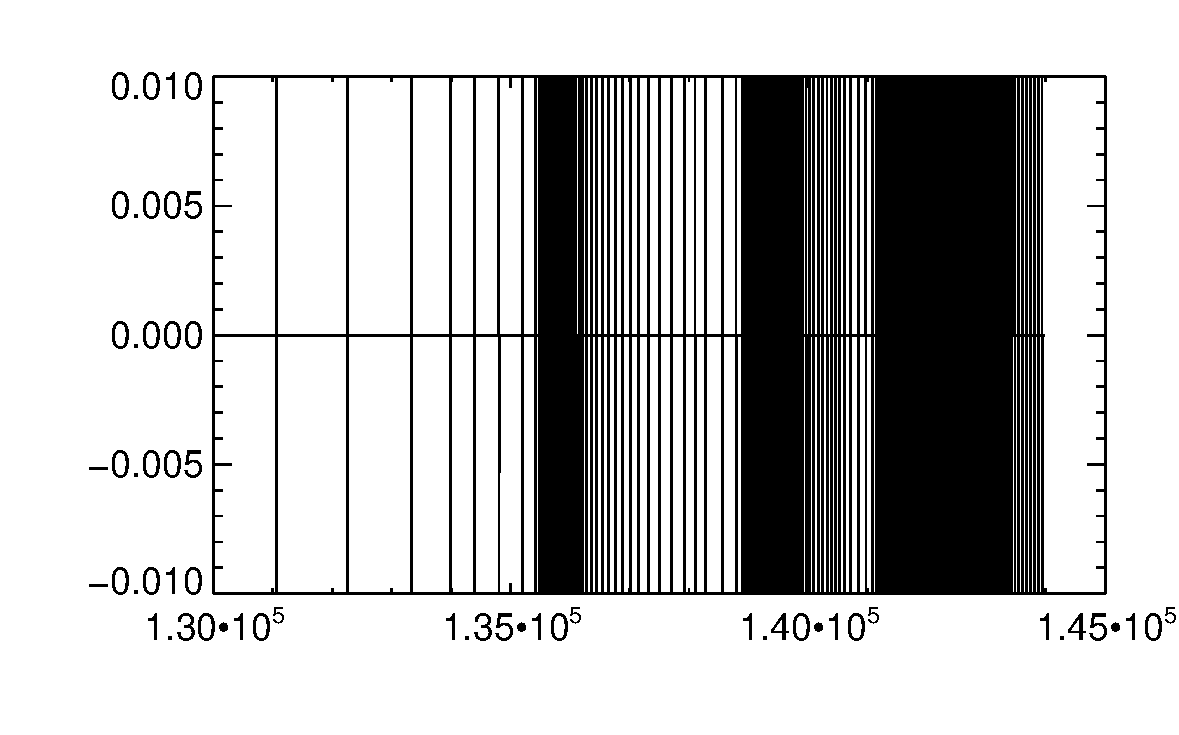
\includegraphics[width=1.\textwidth]{../plots_tables_images/sm_firstsmoothonly.eps}
%         \caption{\hl{\texttt{deriv(deriv(smooth(sortedarray)))}}}
%     \end{subfigure}
%     \begin{subfigure}[b]{.49\textwidth}
%         \centering
%         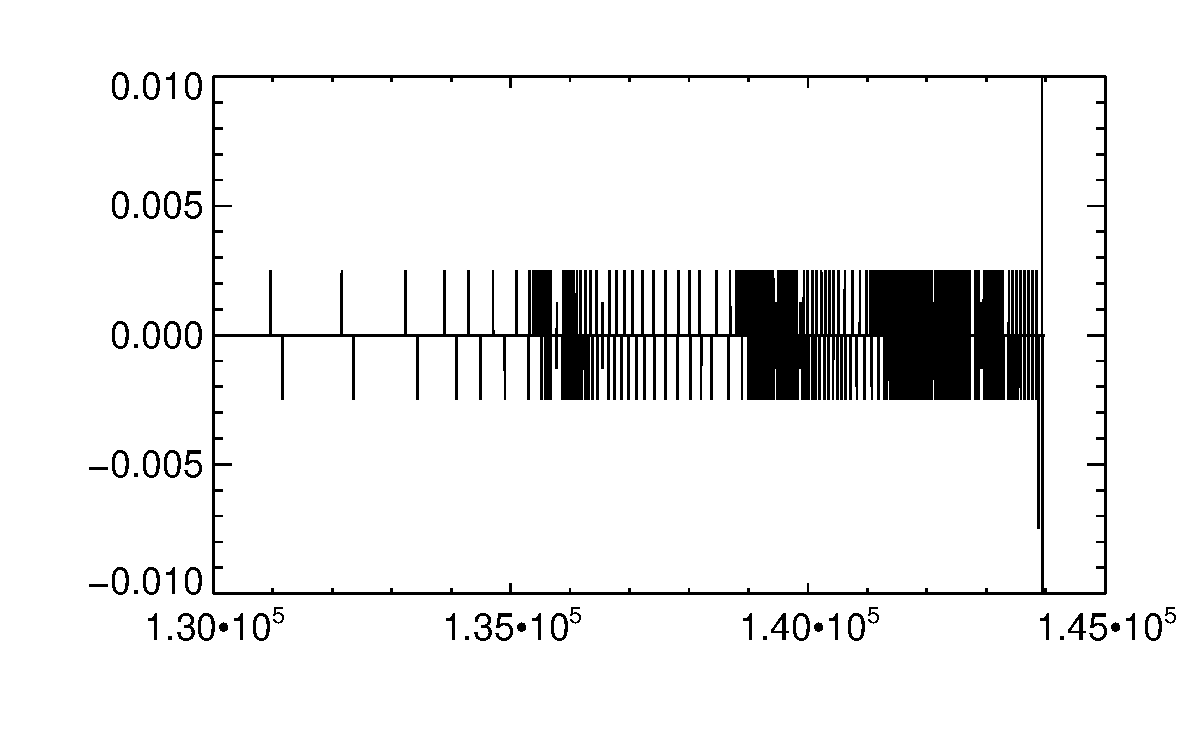
\includegraphics[width=1.\textwidth]{../plots_tables_images/sm_nowrap.eps}
%         \caption{\hl{\texttt{deriv(smooth(deriv(smooth(sortedarray))))}}}
%     \end{subfigure}

%    \begin{subfigure}[b]{.49\textwidth}
%         \centering
%         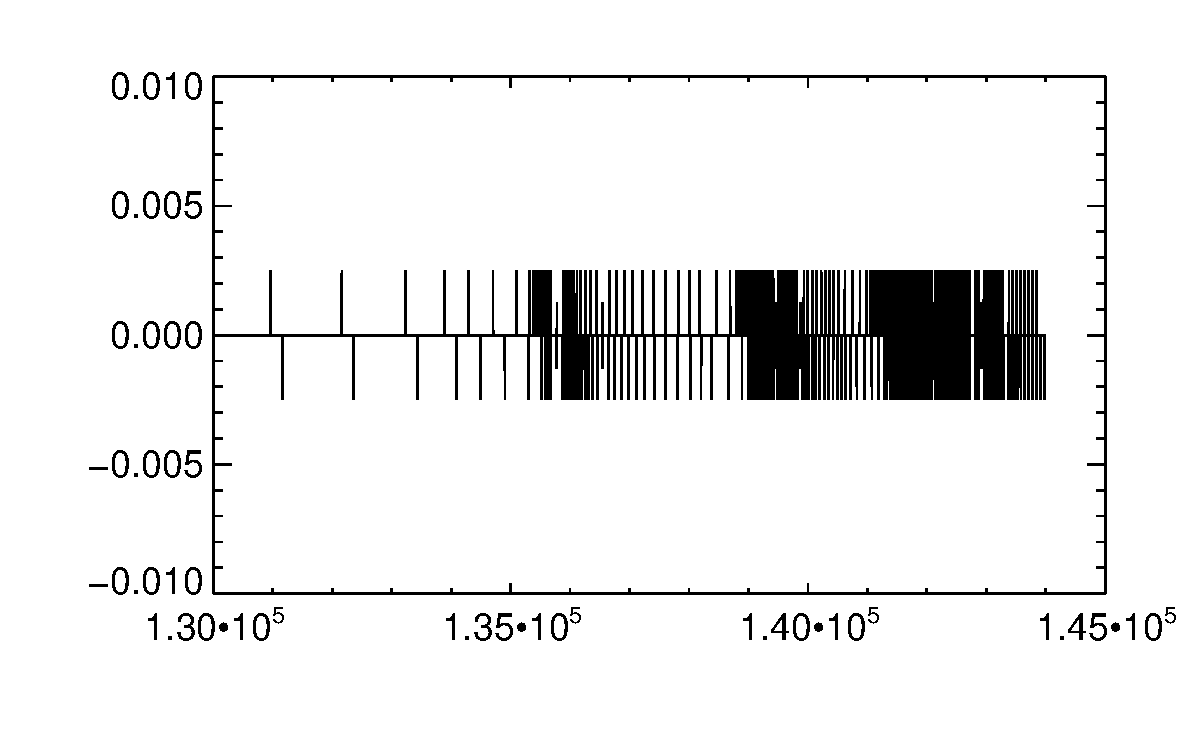
\includegraphics[width=1.\textwidth]{../plots_tables_images/sm_justsmooth.eps}
%         \caption{\hl{\texttt{deriv(smooth(\\
%         deriv(smooth(sortedarray)),/edge\_wrap))}}}
%     \end{subfigure}
%     \begin{subfigure}[b]{.49\textwidth}
%         \centering
%         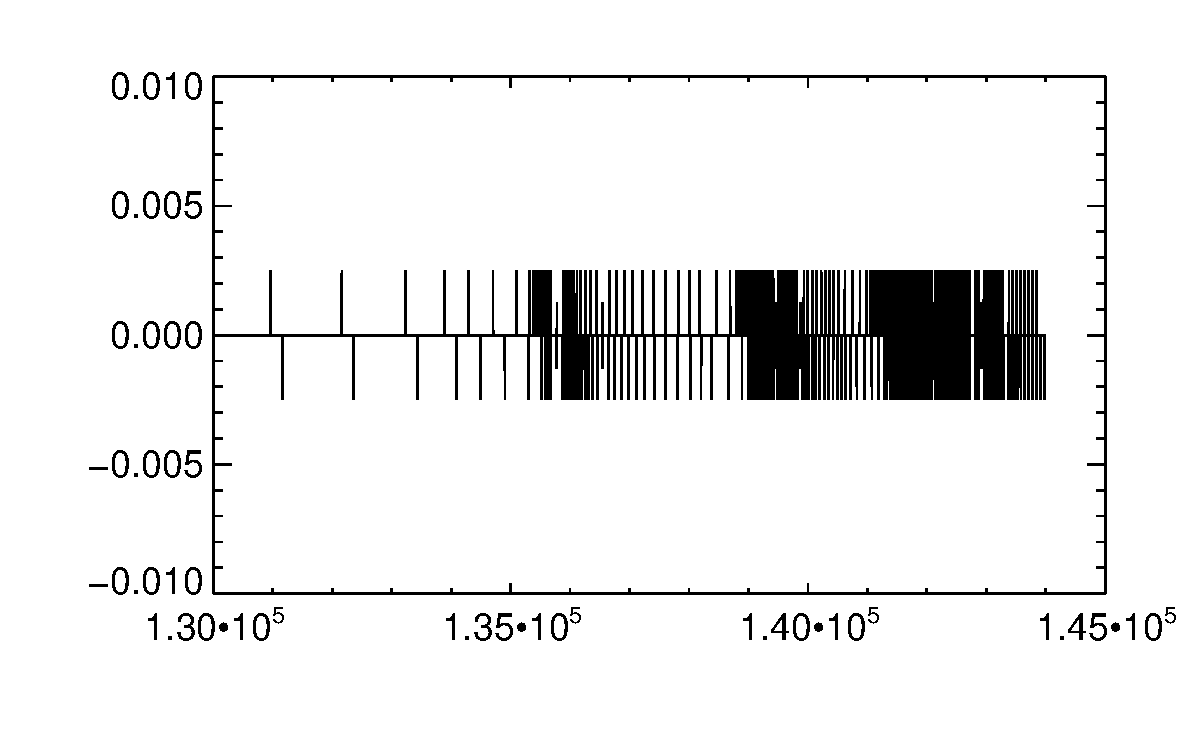
\includegraphics[width=1.\textwidth]{../plots_tables_images/sm_doubletssmooth.eps}
%         \caption{\hl{\texttt{deriv(ts\_smooth(\\
%         deriv(smooth(sortedarray))))}}}
%     \end{subfigure}
%     \caption{}    
%     \label{badsmooth}
%     \end{center}
% \end{figure}

We need a faster way to find the peaks, either through an alternative smoothing method or a new peak-finding method.\\

The current method of associating a region number to a sun is using IDL's \hl{\texttt{label\_region}} and \hl{\texttt{histogram}}. In the future we are going to port over the code from IDL to C++ so I shouldn't rely so heavily on complicated built-in IDL functions. As of now, however, the code is fully functional and further development will be halted in favor of working on other parts of the project. \\

Furthermore, we need to figure out the distinguishing factor that identifies if there is some ``global'' darkening that affects the entire image. The reason is that if we have one image of a 100\% and 50\% sun in some shade that results in an image that \emph{looks} like a 50\% and 25\% sun, how do we tell the difference? \\

We have yet to investigate this issue, but there is a possibility that a fiducial may lie on the edge of the solar limb where we are taking strips of data and muck up our polynomial fitting. We have not seen how much of an effect it would have or if it should be something we are worried about at all. One possible solution is if the program notices a fiducial when trying to fit a polynomial to the solar limb, that it look at the next column/row over until the fiducial doesn't interfere with the data.\\

Currently we are using 5 chords, separated by 5 pixels apart, these are rather arbitrary numbers, perhaps I should do a case study that looks at the optimal numbers to use. Actually, a case study of all the parameters I use, but since we're halting development on the code, this may not happen in the near future. 


\begin{figure}[!ht]
    \centering
    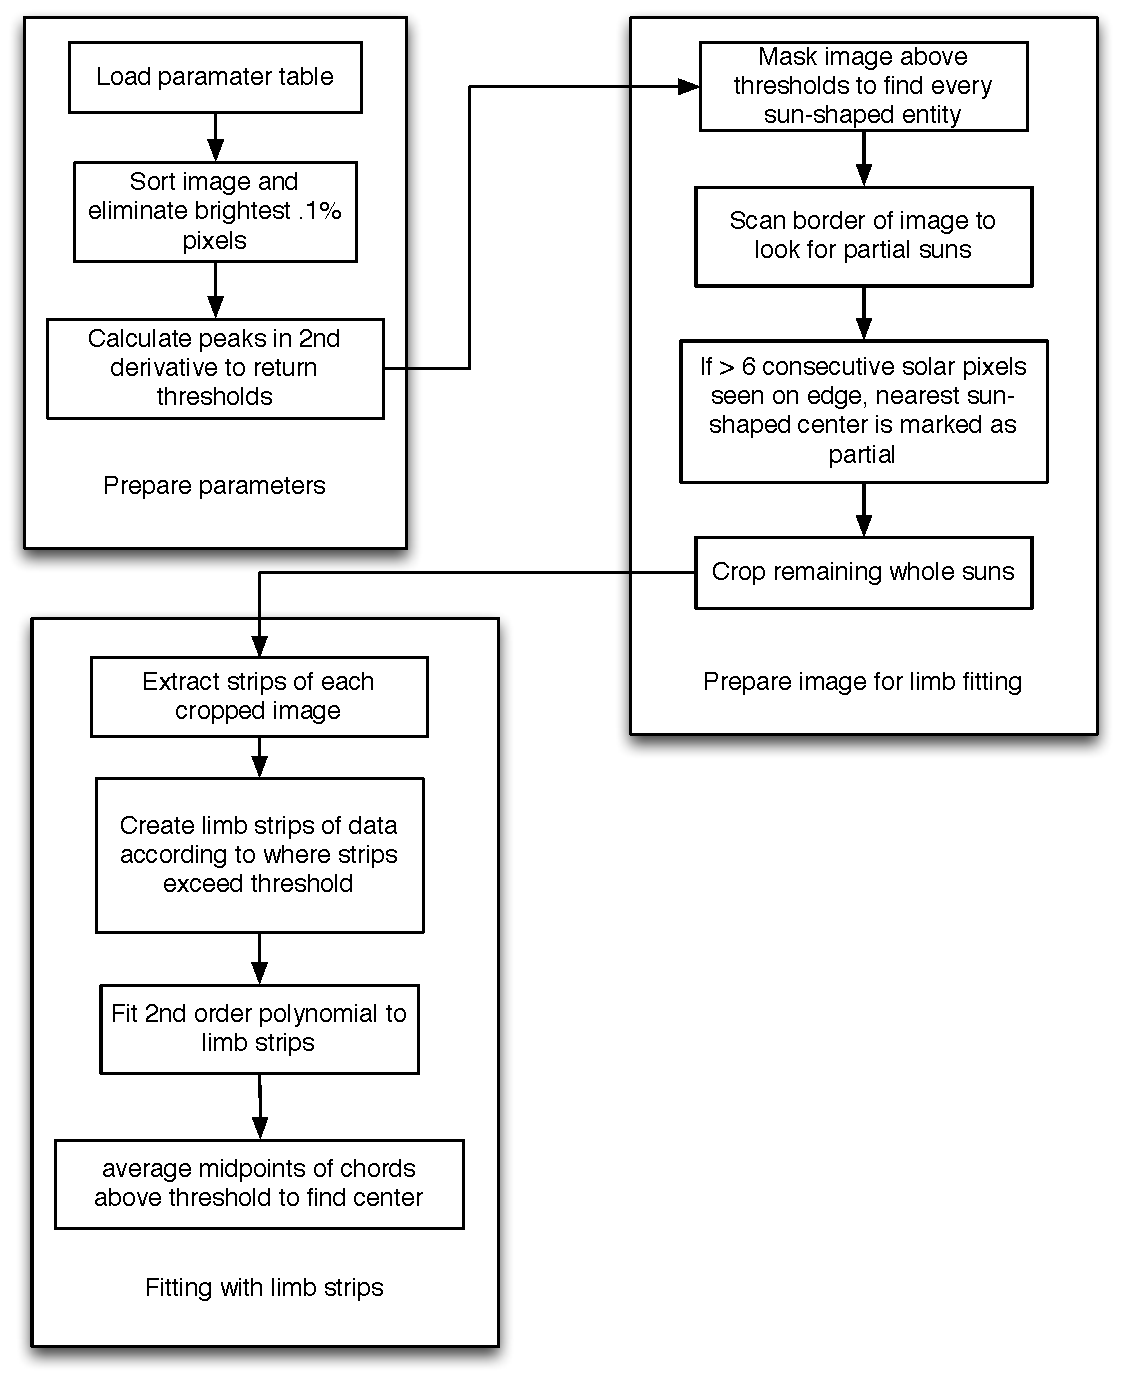
\includegraphics[width=.9\textwidth]{../plots_tables_images/beta_flowchart.pdf}    
\end{figure}

% section issues (end)

\section{Psuedo Issues} % (fold)
\label{sec:psuedo_issues}

One recurring topic that is brought up with each iteration of this software is how fast/accurate it is. The problem is that we don't have a baseline ``This is where the center actually is'' location of the solar centers. This makes it difficult to see how accurate our results are. We have compared limb-fitted results to simple mask-centroiding results to gauge accuracy, although a more reliable centroiding function may involve fitting the solar data to a 2D Gaussian. 
% section psuedo_issues (end)

\end{document}










